\section{同伦}
\label{sec:homol-homotopy}

同胚要求两个空间的点一一对应，并且对应在两个方向上都连续。这个要求很严，常常把我们心目中“形状相同”的空间分开。下面比较平面中的单位圆周和环带，二者都取欧氏空间的子空间拓扑：
\[
 S^1=\{\bm x\in\mathbb R^2:\lVert\bm x\rVert_2=1\},\qquad
 A=\{\bm x\in\mathbb R^2:1\leq\lVert\bm x\rVert_2\leq2\}.
\]

两者都围着同一个洞，但它们不同胚。区分的办法是看去掉两个点之后还剩下什么。图~\ref{fig:homol-remove-two-points}画出了这两种情形。

\begin{BookInlineFigure}
  \centering
  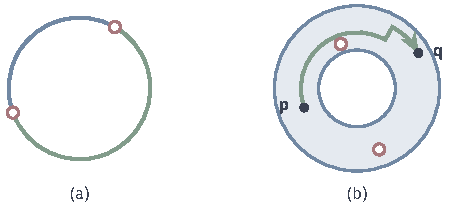
\includegraphics[width=76.962mm]{figures/04-spaces-measures-and-geometry/01-topology-and-metric/tikz/homol-remove-two-points/figure.pdf}
  \caption{圆周与环带各去掉两个点（红色空心点）。(a)圆周断成蓝、绿两段互不相连的开弧。(b)环带中任意两点$\bm p,\bm q$仍可相连：绿色路径先沿圆弧绕到一条避开去掉点的射线，沿射线移动，再沿另一段圆弧到达$\bm q$。}
  \label{fig:homol-remove-two-points}
\end{BookInlineFigure}

从$S^1$中去掉两个不同的点，剩下两段互不相交的开弧，空间不连通。从$A$中去掉任意两点，剩下的部分却仍然路径连通，理由如下。

任取剩下的两点$\bm p,\bm q$。去掉的两点只占两个半径值，所以可以在$\lVert\bm p\rVert_2$附近取一个半径$r_p\in[1,2]$，使半径为$r_p$的圆避开去掉的点，并且从$\bm p$沿半径走到这个圆的短线段也避开它们。对$\bm q$同样取$r_q$。

去掉的点只占两个方向，所以还可以取一条不经过它们的射线。于是从$\bm p$出发沿短线段到半径为$r_p$的圆，沿圆走到射线上，沿射线走到半径为$r_q$的圆，沿这个圆走到$\bm q$的半径方向，最后沿短线段到达$\bm q$。各段首尾相接，就得到一条连接$\bm p,\bm q$的路径。

同胚把“去掉两点”对应为“去掉两点”，并且保持连通性（第~\ref{chap:topological-spaces}章）。两种结果不同，所以$S^1$与$A$不同胚。

可是环带能沿半径连续地压到圆周上，压缩中洞始终存在。要表达“有同样的洞”，需要一种比同胚宽松的比较：不再要求点一一对应，只要求能用连续变形相互转化。下面先定义映射之间的连续变形，再说明怎样把空间连续收回它的子空间。

\subsection{同伦等价}
\label{sec:homol-homotopy-equivalence}

把环带压到圆周上，可以想成一段动画：时间$t$从$0$走到$1$，$t=0$时每个点都在原处，$t=1$时每个点都落到圆周上，中间每一帧都是一个映射。动画要“不跳帧”，不能只要求每一帧连续，还要求同一个点的位置随时间连续变动。

把时间当作一个额外的坐标，这两种连续性就合成了一个条件：动画是定义在“空间$\times$时间”上的一个连续映射。

\begin{definition}[同伦]
\label{def:homol-homotopy}
设$X,Y$为拓扑空间，$f,g:X\to Y$连续，$X\times[0,1]$取乘积拓扑。若存在连续映射$H:X\times[0,1]\to Y$，使得
\begin{equation}
 H(x,0)=f(x),\qquad H(x,1)=g(x),\qquad x\in X,
 \label{eq:homol-homotopy}
\end{equation}
则称$f$与$g$\term{同伦}（homotopy），记为$f\simeq g$，称$H$为从$f$到$g$的一个同伦。
\end{definition}

记$h_t=H(\cdot,t)$，这是动画在时刻$t$的一帧。从图~\ref{fig:homol-homotopy-family}可以同时读出同伦的两种看法：横着看，$X\times[0,1]$的每条水平线给出一个映射$h_t$；竖着看，每条竖线给出一个点$x$的运动轨迹$t\mapsto h_t(x)$。

\begin{BookInlineFigure}
  \centering
  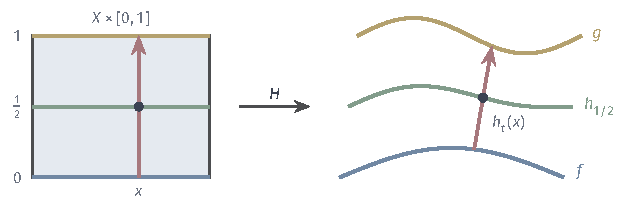
\includegraphics[width=105.971mm]{figures/04-spaces-measures-and-geometry/01-topology-and-metric/tikz/homol-homotopy-family/figure.pdf}
  \caption{同伦把矩形$X\times[0,1]$映到$Y$（此处$X$为线段，$Y$为平面）。蓝、绿、黄三条水平线分别对应$f$、$h_{1/2}$与$g$；红色竖线是固定$x$时的轨迹，它被$H$送成从$f(x)$到$g(x)$的一条路径。}
  \label{fig:homol-homotopy-family}
\end{BookInlineFigure}

$H$在乘积空间上整体连续，比每个$h_t$连续更强。例如令$h_0$为$\mathbb R$上的恒等映射，$t>0$时$h_t$恒取$0$，则每一帧都连续，点$x\neq0$却在$t=0$的瞬间跳到$0$。这样的“跳帧”被整体连续的要求排除了。

最常用的同伦是直线同伦。若$Y\subseteq\mathbb R^n$是凸集，$f,g:X\to Y$连续，令
\begin{equation}
 H(x,t)=(1-t)f(x)+tg(x).
 \label{eq:homol-straight-line-homotopy}
\end{equation}
凸性保证线段上的点仍在$Y$中；$H$由连续函数经乘法与加法得到，因而连续。所以进入凸集的任意两个连续映射都同伦，特别地，进入凸集的映射都同伦于常值映射。

\paragraph{同伦关系的性质}
后面要把同伦的映射看作“同一类”，因此先确认同伦是等价关系，并且与复合相容。

\begin{lemma}[同伦是等价关系]
\label{lem:homol-homotopy-equivalence-relation}
对固定的$X,Y$，连续映射$X\to Y$之间的同伦关系是等价关系。若$f\simeq f':X\to Y$，$g\simeq g':Y\to Z$，则$g\circ f\simeq g'\circ f'$。
\end{lemma}

\begin{proof}
自反性取同伦$H(x,t)=f(x)$，即动画一直停在第一帧。对称性把时间倒过来，若$H$从$f$到$g$，则$H(x,1-t)$从$g$到$f$。

对传递性，设$H$从$f$到$g$，$G$从$g$到$h$。把两段动画接起来，每段用一半时间播放：
\[
 K(x,t)=\begin{cases}H(x,2t),&0\leq t\leq1/2,\\ G(x,2t-1),&1/2\leq t\leq1.\end{cases}
\]
两段在$t=1/2$处都等于$g(x)$，所以$K$有定义。

$K$的连续性用闭集判断。$X\times[0,1/2]$与$X\times[1/2,1]$都是闭集，$K$在其上的限制都连续。对$Y$中任一闭集$F$，$K^{-1}(F)$是两个限制的原像之并。每个原像在相应闭子集中是闭的，因而在整个乘积中是闭的，两个闭集之并仍是闭集，所以$K$连续。

再看与复合的相容性。设$H$从$f$到$f'$，$G$从$g$到$g'$，令
\[
 K(x,t)=G(H(x,t),t).
\]
它是连续映射$(x,t)\mapsto(H(x,t),t)$与$G$的复合，前者的两个分量都连续。代入$t=0$与$t=1$，分别得到$g\circ f$与$g'\circ f'$，所以$K$就是所求的同伦。
\end{proof}

\paragraph{同伦等价与可缩空间}
同胚要求存在互逆的连续映射：去了再回来，恰好回到原处。把“恰好回到原处”放宽为“能连续变回原处”，就得到需要的比较。

\begin{definition}[同伦等价]
\label{def:homol-homotopy-equivalent}
若连续映射$f:X\to Y$与$g:Y\to X$满足
\begin{equation}
 g\circ f\simeq\operatorname{id}_X,\qquad f\circ g\simeq\operatorname{id}_Y,
 \label{eq:homol-homotopy-equivalence}
\end{equation}
则称$f$是\term{同伦等价}（homotopy equivalence），$g$是它的同伦逆，并称$X$与$Y$同伦等价，记为$X\simeq Y$。与单点空间同伦等价的空间称为\term{可缩空间}（contractible space）。
\end{definition}

同胚是同伦等价：互逆映射的复合恰好等于恒等映射。同伦等价的复合仍是同伦等价。设$f:X\to Y$的同伦逆为$g$，$f':Y\to Z$的同伦逆为$g'$，由引理~\ref{lem:homol-homotopy-equivalence-relation}的复合相容性，
\[
 (g\circ g')\circ(f'\circ f)=g\circ(g'\circ f')\circ f
 \simeq g\circ\operatorname{id}_Y\circ f=g\circ f\simeq\operatorname{id}_X,
\]
另一侧同理。所以空间之间的同伦等价也是等价关系。

可缩性有一个更直接的判据：$X$可缩，当且仅当$\operatorname{id}_X$同伦于某个常值映射。设$X\simeq\{p\}$，映射为$f:X\to\{p\}$，同伦逆$g$把$p$送到某点$x_0$，则$g\circ f$是取值$x_0$的常值映射，它同伦于$\operatorname{id}_X$。

反过来，若$\operatorname{id}_X$同伦于取值$x_0$的常值映射，取$f:X\to\{p\}$与$g(p)=x_0$。此时$g\circ f$正是这个常值映射，而$f\circ g=\operatorname{id}_{\{p\}}$自动成立。

\begin{example}[区间与圆盘可缩]
\label{ex:homol-contractible}
闭圆盘是含原点的凸集，记为
\[
 D^2=\{\bm x\in\mathbb R^2:\lVert\bm x\rVert_2\leq1\}.
\]
取直线同伦
\[
 H(\bm x,t)=(1-t)\bm x,
\]
它从恒等映射连续变到取值为原点的常值映射，所以圆盘可缩。例如点$(1,0)$在$t=1/2$时位于$(1/2,0)$，在$t=1$时到达原点。同样的公式把$[-1,1]$收缩到原点。对一般的非空凸集，任取其中一点$\bm a$，用$H(\bm x,t)=(1-t)\bm x+t\bm a$，所以区间$[0,1]$、$\mathbb R^n$及其中任何非空凸集都可缩。
\end{example}

环带是否可缩，直观上似乎一目了然：中间的洞消不掉。但要证明不存在从$\operatorname{id}_A$到常值映射的同伦，就要排除所有可能的连续变形，一个个去试做不到。这正是同调要解决的问题，第~\ref{sec:homol-homotopy-invariance}小节将给出证明。

\paragraph{同伦等价与同胚的区别}
同伦等价比同胚宽松得多。单点与区间$[0,1]$同伦等价，却不同胚，因为两者之间连双射都没有。区间与圆盘都可缩，因而同伦等价，但它们也不同胚。

区间去掉一个内点就不连通。圆盘去掉任何一点$\bm q$却仍然路径连通：任取剩下的两点，取一点$\bm m\in D^2$，使它不在过这两点的直线上；由凸性，两条线段经过$\bm m$把这两点连起来，而除这两点外它们都不在那条直线上，碰不到$\bm q$（$\bm q$若不在这条直线上，直接取线段即可）。同胚把“去掉一点”对应为“去掉一点”，所以二者不同胚。

\begin{BookInlineTable}
  \centering
  \caption{同胚与同伦等价的比较}
  \label{tab:homol-homeo-vs-homotopy}
  \begin{tabular}{lll}
    \toprule
    & 同胚 & 同伦等价 \\
    \midrule
    需要的映射 & 互逆的$f,g$ & 复合同伦于恒等映射的$f,g$ \\
    点的对应 & 一一对应 & 可以把一片压成一点 \\
    保持的信息 & 维数、局部形状等 & 连通分支、洞的个数等 \\
    区间与单点 & 不同 & 相同 \\
    环带与圆周 & 不同 & 相同 \\
    \bottomrule
  \end{tabular}
\end{BookInlineTable}

表~\ref{tab:homol-homeo-vs-homotopy}把两种比较放在一起。同伦等价忽略了维数和点的多少，只保留连续变形下不变的整体信息。表中“保持的信息”一行里的“洞的个数”，还需要用本章后面的同调来说清楚。

\subsection{形变收缩}
\label{sec:homol-deformation-retraction}

环带压向圆周的过程有一个特点：圆周上的点始终不动，其余的点最终都落到圆周上。这样的变形把空间收回到它的一个子空间，而子空间本身不受扰动。

把这个过程拆成两件事：最后的结果是一个把空间收回子空间的映射，过程是把这个映射与恒等映射连起来的同伦。

\begin{definition}[形变收缩]
\label{def:homol-deformation-retraction}
设$Y\subseteq X$为子空间。若连续映射$r:X\to Y$满足$r(a)=a$对一切$a\in Y$成立，则称$r$为\term{回缩}（retraction）。若存在连续映射$H:X\times[0,1]\to X$，满足
\begin{align}
 H(x,0)&=x,\quad H(x,1)\in Y,&x&\in X,\label{eq:homol-deformation-end}\\
 H(a,t)&=a,&a&\in Y,\ t\in[0,1],\label{eq:homol-deformation-fixed}
\end{align}
则称$H$为从$X$到$Y$的\term{形变收缩}（deformation retraction），称$Y$为$X$的形变收缩核。
\end{definition}

两条要求分工不同。式~\eqref{eq:homol-deformation-end}说变形从恒等映射出发，终点落在$Y$中；式~\eqref{eq:homol-deformation-fixed}说$Y$上的点全程固定。两条合起来，终止映射$r=H(\cdot,1)$满足$r|_Y=\operatorname{id}_Y$，是一个回缩；而$H$本身是从$\operatorname{id}_X$到$i\circ r$的同伦，其中$i:Y\to X$是包含映射。

\begin{example}[环带收向圆周]
\label{ex:homol-annulus-retraction}
对环带$A$与圆周$S^1$，令
\begin{equation}
 H(\bm x,t)=(1-t)\bm x+t\frac{\bm x}{\lVert\bm x\rVert_2}.
 \label{eq:homol-annulus-retraction}
\end{equation}
在$A$上$\lVert\bm x\rVert_2\geq1$，分母不为零，所以$H$连续。$H(\bm x,t)$与$\bm x$同方向，长度为
\[
 \lVert H(\bm x,t)\rVert_2=(1-t)\lVert\bm x\rVert_2+t\in[1,2],
\]
所以始终留在$A$中。

$t=0$时$H$是恒等映射。$t=1$时它把每点沿半径送到圆周上，例如点$(0,2)$在$t=1/2$时位于$(0,3/2)$，在$t=1$时到达$(0,1)$。若$\lVert\bm x\rVert_2=1$，则$H(\bm x,t)=\bm x$，圆周上的点不动。因此$H$是从$A$到$S^1$的形变收缩。同一公式也把去掉原点的平面$\mathbb R^2\setminus\{\bm 0\}$形变收缩到$S^1$。
\end{example}

\begin{BookInlineFigure}
  \centering
  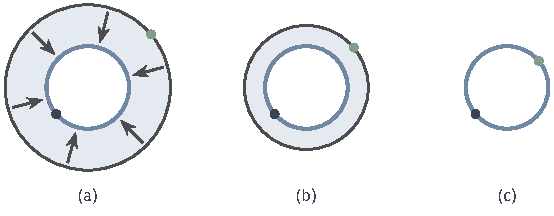
\includegraphics[width=93.832mm]{figures/04-spaces-measures-and-geometry/01-topology-and-metric/tikz/homol-annulus-retraction/figure.pdf}
  \caption{环带沿半径收向圆周，(a)(b)(c)依次是式~\eqref{eq:homol-annulus-retraction}在$t=0,\,1/2,\,1$的像。粗蓝线是单位圆周，全程不动；外缘上的绿点半径由$2$变为$3/2$，再变为$1$；圆周上的黑点始终停在原处。}
  \label{fig:homol-annulus-retraction}
\end{BookInlineFigure}

图~\ref{fig:homol-annulus-retraction}是这个过程的三帧。把它写成一般结论，形变收缩给出的正是同伦等价所需要的那对映射。

\begin{theorem}[形变收缩给出同伦等价]
\label{thm:homol-retract-equivalence}
若$Y$是$X$的形变收缩核，$r=H(\cdot,1)$为相应的回缩，$i:Y\to X$为包含映射，则$i$是同伦等价，$r$是它的同伦逆。特别地，$X\simeq Y$。
\end{theorem}

\begin{proof}
由于$r$在$Y$上是恒等映射，一侧等式严格成立：
\[
 r\circ i=\operatorname{id}_Y.
\]

另一侧，由定义，$H$满足$H(x,0)=x$与$H(x,1)=i(r(x))$，它正是从$\operatorname{id}_X$到$i\circ r$的同伦，所以$i\circ r\simeq\operatorname{id}_X$。
\end{proof}

由例~\ref{ex:homol-annulus-retraction}与定理~\ref{thm:homol-retract-equivalence}，$A\simeq S^1$。环带与圆周不同胚，却同伦等价，这正是本节开头想表达的“有同样的洞”。

\paragraph{回缩本身不够}
只有回缩而没有形变，不能得出同伦等价。取两点离散空间$X=\{0,1\}$与子空间$Y=\{0\}$，常值映射$r\equiv0$是回缩。若$i\circ r\simeq\operatorname{id}_X$，同伦限制在点$1$上就给出一条从$0$到$1$的路径，可是$X$不连通，这样的路径不存在。

所以$Y$不是$X$的形变收缩核。回缩只说“结果”：每个点都有去处。形变收缩还要求“过程”：每个点能沿连续的路径走到去处。上面的点$1$有去处，却没有路可走。

定义要求$Y$全程固定，这比同伦等价所需要的略强。若只要$X\simeq Y$，允许$Y$中的点在$Y$内部移动也够了：此时$H$限制在$Y$上给出$r\circ i\simeq\operatorname{id}_Y$，定理~\ref{thm:homol-retract-equivalence}的结论不变。保留固定条件，是因为它描述的正是“把多余部分收回、核心不动”这一具体过程；第~\ref{chap:manifold-recovery}章把点云邻域收回流形时，用的就是这种形式。

同伦等价究竟保留了什么代数信息，需要先建立同调才能回答。下一节先解决输入的问题：怎样把一个空间写成有限的数据。
